\documentclass[11pt]{article}

\usepackage[a4paper,margin=2.6cm]{geometry}
\usepackage{fontspec}
\setmainfont{Noto Sans KR}
\usepackage{amsmath,amssymb}
\usepackage{graphicx}
\usepackage{booktabs}
\usepackage{longtable}
\usepackage{xcolor}
\usepackage{hyperref}
\usepackage{tikz}
\usetikzlibrary{arrows.meta,positioning,calc}
\usepackage{caption}
\usepackage{kotex}

\hypersetup{colorlinks=true, linkcolor=blue!50!black, citecolor=blue!50!black, urlcolor=blue!40!black}

\title{\textbf{쉘 후좌굴(Post-Buckling) One-to-Many 벤치마크\\
형상 · Imperfection 법칙 · 예상 출력}}
\author{AI-CAE4ALL --- MeshGraphNets-Variational 검증 벤치마크 설계}
\date{2026년 9월}

\begin{document}
\maketitle

\begin{abstract}
\noindent
얇은 원통형 쉘(shell)은 축방향 압축을 받으면 여러 개의 거의 동등한 좌굴 모드 중
하나로 무너진다. 어느 모드가 선택되는지는 역학적으로는 무시할 만큼 작은
\emph{imperfection}(형상 결함)이 결정한다. 이 벤치마크는 그 imperfection의
\textbf{법칙(law)}만 지정하고 실제 실현값(realization)은 모델에게 숨긴다 --- 즉
모델은 완벽한 원통이라는 공칭(nominal) 형상만 보고 후좌굴 변형장(field)의
\emph{분포}를 예측해야 한다. 우리가 \emph{정하는} 값은 딱 다섯 개다: 반지름
$R$, 두께 $t$, 길이 $L$, 부과 압축량 $\Delta$, 그리고 dimple 깊이 $a$. 앞의
넷은 설계점(design point)의 성질이고, 다섯 번째 $a$만 draw마다 다시 뽑힌다.
다섯 모두 \textbf{하나의 직육면체 박스 위 독립 균일(또는 정규) 분포}이며 ---
조건부 경계도, 기각(rejection)도, 파생량 스윕도 없다. 축하중 $P$는 입력이
아니라 \textbf{출력}이다: 극한점을 지나면 평형 자체가 없으므로 변위 제어로
밀고, $P$는 강체 단면의 반력 이력에서 되읽는다. Imperfection은 표면을 국소적으로
미는 \textbf{Gaussian dimple 단 한 개}($K{=}1$)로 줄여서, 숨겨진 잠재변수가
정확히 3차원 $(a, z, \theta)$이 되도록 만들었다. 재료는
Butterfly~Defect 논문(arXiv:2607.19245)의 Neo-Hookean 초탄성이 아니라
\textbf{선형탄성} 강재($E{=}210$~GPa, $\nu{=}0.3$, $\rho{=}7.85\times10^{-6}$
kg/mm$^3$; kg-mm-ms 단위계)를 쓴다. 이 문서는
(1) 어떤 형상을 다루는지, (2) imperfection이 어떤
방식·어떤 확률적 메커니즘으로 들어가는지, (3) 최종적으로 어떤 출력이
데이터셋에 담기는지를 설명하고, 이 설계를 방법론적으로 참고한
Butterfly~Defect 논문의 실험 설계와 나란히 비교한다.
\end{abstract}

\tableofcontents

% =====================================================================
\section{왜 이런 벤치마크가 필요한가}
% =====================================================================

MeshGraphNets-Variational(MGN-V)은 하나의 입력 형상에 대해 \emph{하나의}
정답이 아니라 \emph{여러 개의 그럴듯한 정답}을 만들어내야 하는 문제를 위한
모델이다. 그런데 이런 모델을 제대로 검증하려면, "같은 입력에 대해 실제로
서로 다른 결과가 나오는" 데이터가 있어야 한다. 이번 세션에서 조사한
결과, 이런 조건을 정확히 만족하는 공개 데이터셋은 존재하지 않는다:

\begin{itemize}
\item ConcreteShellFEA (Bath, 2026)는 imperfection을 \textbf{입력 변수로 노출}한다 ---
      즉 모델이 imperfection 자체를 보고 결과를 맞히면 되므로, one-to-many가 아니라
      평범한 one-to-one 회귀 문제가 되어버린다.
\item Bristol 복합재 원통 데이터셋은 실물 시험편이 2개뿐이라 학습에 쓸 수 없다.
\item Butterfly~Defect 논문 자체는 방법론은 훌륭하지만 데이터나 코드를 공개하지 않았다.
\end{itemize}

그래서 우리가 직접 만든다. 물리적 소재는 얇은 쉘의 축압축 좌굴 --- "결정은
숨겨진 랜덤 변수가 하고, 모델은 그 변수를 볼 수 없다"는 구조가 교과서적으로
성립하는 문제다.

\begin{center}
\begin{tikzpicture}[node distance=8mm, every node/.style={font=\small}]
  \node[draw, rounded corners, minimum width=3.6cm, minimum height=1.0cm, align=center] (geo)
       {완벽한 원통 $(R,t,L)$ $+$ 압축량 $\Delta$\\(모델이 보는 입력)};
  \node[draw, dashed, rounded corners, minimum width=3.6cm, minimum height=1.0cm, align=center,
        right=of geo, fill=red!5] (imp)
       {Dimple 실현값 $(a, z, \theta)$\\\textbf{(숨김, withheld)}};
  \node[draw, rounded corners, minimum width=3.0cm, minimum height=1.0cm, align=center,
        below=of $(geo)!0.5!(imp)$] (fea)
       {비선형(형상) FEA solve\\(OpenRadioss, 선형탄성)};
  \node[draw, rounded corners, minimum width=4.4cm, minimum height=1.0cm, align=center,
        below=of fea, fill=blue!5] (out)
       {최종 변위장 $p(\text{field} \mid \text{geo})$\\여러 draw $=$ 여러 좌굴 모드};
  \draw[-Latex] (geo) -- (fea);
  \draw[-Latex] (imp) -- (fea);
  \draw[-Latex] (fea) -- (out);
\end{tikzpicture}
\end{center}

이 구조에서 "one-to-many"는 그림의 점선 상자를 모델에게 숨기는 데서 전부
나온다. Dimple 실현값을 숨기지 않고 입력으로 준다면, 이 문제는 즉시 결정론적
회귀 문제로 붕괴한다 --- 이것이 바로 위에서 언급한 기존 공개 데이터셋들의
공통된 실패 지점이다. 입력 쪽은 일부러 아무 것도 감추지 않는다: 완벽한 원통은
$R,t,L$ 세 숫자로 완전히 결정되고 하중 조건은 압축량 $\Delta$ 하나가 전부이므로,
모델이 보는 입력에는 모호함이 전혀 없다 --- 모호함은 오직 dimple 쪽에서만 온다.
숨겨지는 잠재변수는 정확히 3차원이다: 깊이 $a$, 축방향 위치 $z$, 원주방향
위치 $\theta$.

% =====================================================================
\section{1. 설계 공간 --- 우리가 정하는 다섯 개의 값}
% =====================================================================

형상은 \textbf{단 하나의 계열(family)}만 다룬다: 원형 단면 원통형 쉘. 원뿔이나
두께 테이퍼처럼 파라미터가 더 필요한 형상족은 일부러 두지 않았다 --- 형상
쪽에서 복잡도를 늘리는 것은 이 벤치마크의 목적(imperfection이 만드는
one-to-many 구조를 보는 것)에 도움이 되지 않기 때문이다. 모든 형상은 같은
경계조건(바닥 고정, 상단은 축방향으로만 눌림)과 같은 하중 방향(축압축)을 쓴다.

우리가 \emph{정하는} 값은 전부 다섯 개이고, 다섯 모두 \textbf{하나의 직육면체
박스 위 독립 분포}에서 뽑는다 --- 조건부 경계도, 기각(rejection)도, 파생량
스윕도 없다:

\begin{table}[h]
\centering
\small
\begin{tabular}{@{}cllll@{}}
\toprule
 & 기호 & 의미 & 분포 & 언제 뽑히나 \\
\midrule
1 & $R$      & 반지름   & $\mathcal{U}[100,\,200]$ mm & 설계점마다 \\
2 & $t$      & 두께     & $\mathcal{U}[1.0,\,2.0]$ mm & 설계점마다 \\
3 & $L$      & 길이     & $\mathcal{U}[150,\,300]$ mm & 설계점마다 \\
4 & $\Delta$ & 압축량   & $\mathcal{U}[1.0,\,3.0]$ mm & 설계점마다 \\
\midrule
5 & $a$      & dimple 깊이 & $\mathcal{N}(0,\,0.4^2)$ mm & \textbf{draw마다} \\
\bottomrule
\end{tabular}
\caption{다섯 개의 노브. 앞의 넷은 \textbf{설계점(design point)의 성질}이라
그 설계점의 모든 draw가 같은 값을 공유한다. 다섯 번째 $a$만 draw마다 다시
뽑히며, 부호가 곧 바깥쪽/안쪽 dimple이다. 축하중 $P$는 여기에 없다 --- $P$는
입력이 아니라 출력이기 때문이다(아래 참조).}
\end{table}

\noindent
\textbf{왜 $P$가 노브가 아닌가.} 좌굴의 극한점을 지나면 같은 하중을 지탱하는
평형 상태 자체가 없어진다. 하중 제어로 밀면 해석은 극한점에서 발산해버리고,
우리가 보고 싶은 후좌굴 변형장은 아예 나오지 않는다. 그래서 \textbf{변위 제어}로
민다: 상단을 $\Delta$만큼 눌러 내리고, 축하중 $P$는 그 결과로 \emph{측정}한다
(3절). 즉 $P$는 데이터셋의 출력이지 입력이 아니며, 우리가 보고하는 knockdown
factor는 측정된 $P_{\max}$를 고전 임계하중 $P_{cr}$로 나눈 값이다.

\begin{figure}[h]
  \centering
  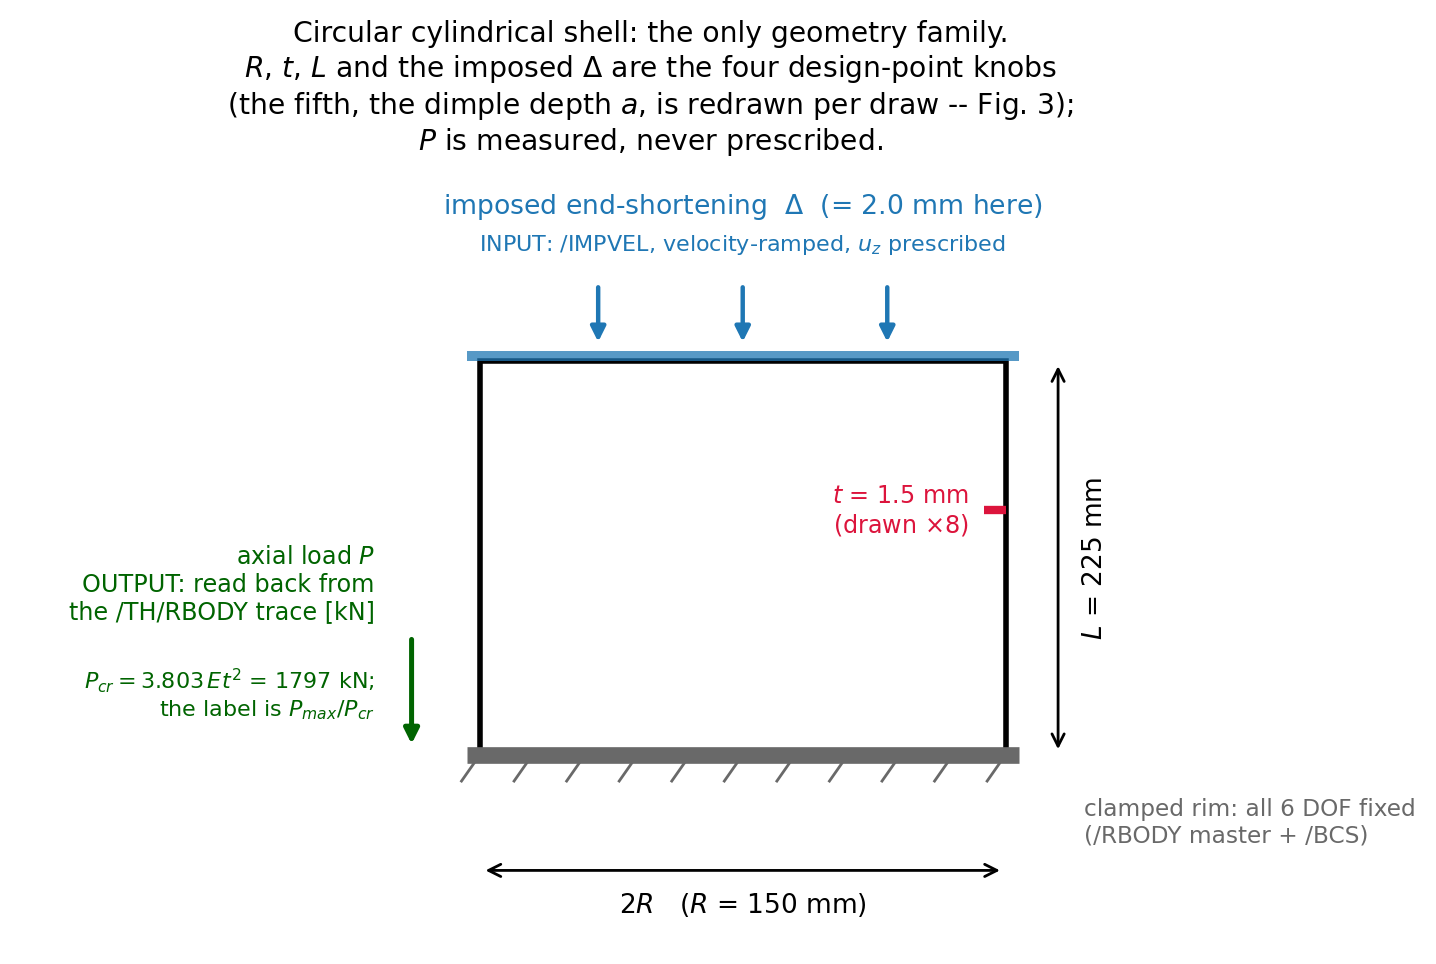
\includegraphics[width=0.62\textwidth]{figures/geometry_schematic.png}
  \caption{다루는 유일한 형상: 원형 원통형 쉘. 바닥 림은 완전 고정, 상단 림은
  강체로 묶어 축방향으로 $\Delta$만큼 눌러 내린다($\Delta$가 \textbf{입력}).
  축하중 $P$는 그 강체 단면의 반력에서 \textbf{읽어낸다}(출력, kN).}
\end{figure}

\begin{figure}[h]
  \centering
  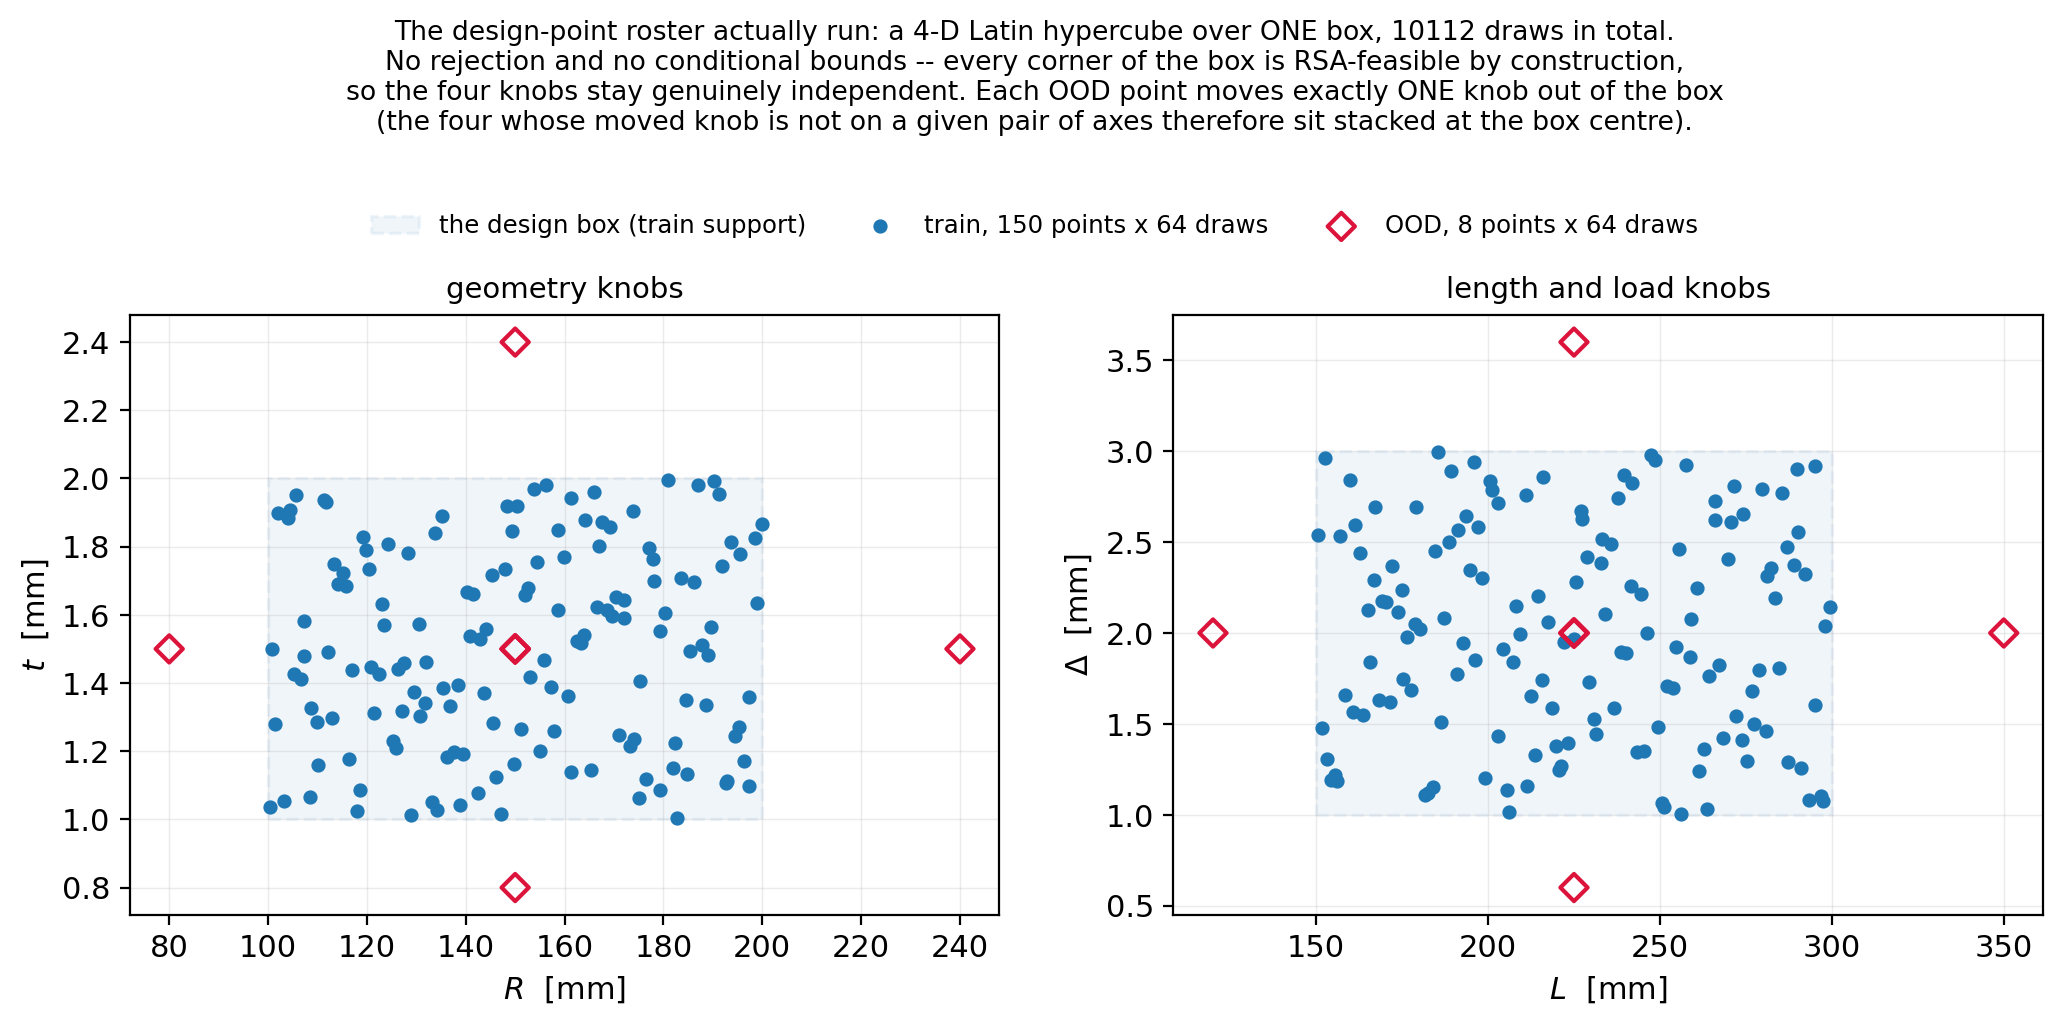
\includegraphics[width=0.98\textwidth]{figures/design_box.png}
  \caption{설계점 로스터. 학습 티어 150점은 4차원 박스 $[100,200]\times
  [1.0,2.0]\times[150,300]\times[1.0,3.0]$ 위의 라틴 하이퍼큐브(LHS)에서 뽑고,
  외삽 티어 8점은 박스 중심 $(R,t,L,\Delta) = (150,\,1.5,\,225,\,2.0)$에서
  \textbf{한 축씩만} 범위 밖으로 밀어낸 점이다 --- 어느 축의 외삽이 실패를
  일으켰는지가 곧바로 읽히도록. 설계점당 64 draw이므로 총
  $158 \times 64 = 10{,}112$ draw다.}
\end{figure}

\noindent
외삽 축은 각각 $R\in\{80,240\}$, $t\in\{0.8,2.4\}$, $L\in\{120,350\}$,
$\Delta\in\{0.6,3.6\}$ mm이다. 한 번에 한 축만 움직이므로, t1에서 성능이
떨어졌을 때 "무엇이 낯설어서" 떨어졌는지가 축 이름 하나로 특정된다. 형상족은
항상 같고 오직 값만 학습 범위 밖으로 나간다.

박스에 걸리는 제약은 단 하나, 물리적 타당성 조건이다: dimple이 경계층 효과와
섞이지 않으려면 원통이 충분히 길어야 한다. Dimple 중심을 양 끝에서 $2\sigma$
이상 떼어놓아야 하므로(2.2절) $L > 4\,l_c(R,t) = 6.914\sqrt{Rt}$가 필요하다.
위의 박스는 이 조건을 \textbf{기각 없이} 만족한다 --- 가장 빡빡한 구석
($L{=}150$, $R{=}200$, $t{=}2.0$)에서도 여유가 $L/L_{\min} = 1.157$이다. 그래서
샘플링에 조건부 경계가 필요 없고, 다섯 노브는 서로 완전히 독립이다.

% =====================================================================
\section{2. Imperfection --- 어떤 방식으로, 어떤 랜덤으로 들어가는가}
% =====================================================================

가장 중요한 설계 지점이다. 공칭 형상은 \textbf{완벽한 원통}이다 --- 그 자체로는
imperfection이 전혀 없고, $R,t,L$로 완전히 결정된다. Imperfection은 그 위에
얹는 단 하나의 법칙으로만 들어간다: 표면을 국소적으로 안쪽 또는 바깥쪽으로
밀어내는 \textbf{단 하나의 Gaussian dimple}($K{=}1$). 즉 "노드들을 안쪽으로
밀거나 밖으로 빼는" 가장 단순한 아이디어를, 메쉬 해상도에 무관하도록
(mesh-independent) 매끄럽게 만든 것이 전부다. 이 방식은 Butterfly~Defect 논문이
실제 실리콘 쉘에 결함을 낼 때 쓴 방법과 그대로 같다.

$K{=}1$은 의도적인 축소다. Dimple을 하나로 줄이면 숨겨진 잠재변수가 정확히
3차원 $(a, z, \theta)$이 되어, "모델이 몇 차원짜리 모호함을 못 보고 있는가"가
애매하지 않게 정의된다. 하나로 줄여도 knockdown 산포는 그대로 나온다는 것은
사전 검증(\texttt{k1\_verify})에서 확인했다 --- 좌굴 개시는 결국 가장 불리한
결함 \emph{하나}가 결정하기 때문이다.

\subsection{Dimple 하나의 모양}

원통 표면을 $(\theta, z)$로 펼쳤을 때, $k$번째 dimple이 표면을 미는 양은
\[
  w_k(\theta, z) = a_k \exp\!\left(-\frac{d_k(\theta,z)^2}{\sigma^2}\right),
  \qquad
  d_k(\theta,z)^2 = \big(R\,\Delta\theta_k\big)^2 + (z - z_k)^2,
\]
이다. 여기서 $\Delta\theta_k$는 $\theta$와 dimple 중심 $\theta_k$ 사이의
(원주를 따라 감긴) 최단 각도 차이다. 폭 $\sigma$는 \textbf{형상마다 고정된
값}이지만, 임의의 상수가 아니라 Butterfly~Defect 논문이 실제로 쓰는 고전적
축대칭 좌굴 반파장(half-wavelength)에서 그대로 가져온다:
\[
  \sigma \;=\; l_c \;=\; \pi\,\big[12(1-\nu^2)\big]^{-1/4}\sqrt{Rt}
  \qquad \text{(원 논문 Eq.~3)},
\]
재료의 $\nu = 0.3$(3절)를 넣으면 $l_c \approx 1.73\sqrt{Rt}$이다. $l_c$는
$R$과 $t$ \textbf{둘 다}에 의존하므로, 같은 $R$에서 $t$가 얇아질수록(즉 $R/t$가
커질수록) $\sigma/R$도 자동으로 줄어든다 --- 만약 $\sigma$를 $R$만의 고정
비율(예: $\sigma = 0.11R$)로 두면, 얇은 쉘일수록 dimple이 반파장에 비해
상대적으로 너무 넓어져 버려서 우리 설계 박스(표 1)의 양 끝에서 물리적으로
다른 크기의 결함을 만드는 셈이 된다. $\sigma=l_c$로 두면
이 문제가 없다: Butterfly~Defect 논문에서 defect 모양 파라미터
$a{=}1,\lambda{=}1$을 고정하면 원주·축 방향 반폭이 정확히 $l_c$가 되므로
(Sec.~II, Eq.~4), 우리 $\sigma$는 그 값을 그대로 재현한 것이다. 메쉬 요소
크기는 항상 $\sigma$의 10분의 1 이하로 잡는다 --- 이 여유가 있어야 메쉬를
조밀하게 해도 dimple의 모양 자체가 바뀌지 않는다. 이 고정은 우리만의 선택이
아니다: Butterfly~Defect 논문의 확률적 multi-defect 실험(Sec.~VI) 역시 defect
모양 파라미터 $(a,\lambda)$를 draw 내내 고정값($a{=}1,\lambda{=}1$)으로 두고
위치와 진폭만 무작위화한다 --- 폭 자체를 바꾸는 실험은 별도의 결정론적
스윕(Sec.~IV)이지, 확률적 앙상블 안에서 defect마다 다시 뽑는 변수가 아니다.
구현은 일반적인 $K$개 dimple의 합을 그대로 두되,
\[
  w(\theta, z) = \sum_{k=1}^{K} w_k(\theta, z),
\]
프로덕션 캠페인은 $K{=}1$로 돌린다. 박스 중심 $(R,t) = (150,\,1.5)$에서
$\sigma = l_c = 25.92$ mm이고, 메쉬 요소 크기는 박스 전체에서
$h/l_c \in [0.083,\,0.084]$로 위의 $1/10$ 상한을 항상 만족한다.

\subsection{무엇이, 어떻게 랜덤인가}

한 설계점 안의 매 draw마다 독립적으로 다음 \textbf{세 개}를 새로 뽑는다 ---
그리고 이 셋이 숨겨진 잠재변수의 전부다:

\begin{itemize}
\item \textbf{깊이 $a$} (설계 노브 5번): 물리 단위 mm로 직접
      $a \sim \mathcal{N}(0,\,\sigma_a^2)$, $\sigma_a = 0.4$ mm에서 뽑는다.
      부호가 곧 방향이다 --- $a>0$이면 바깥쪽으로 부푼 dimple, $a<0$이면
      안쪽으로 눌린 dimple이고, 정규분포는 대칭이므로 두 방향이 자동으로
      반반씩 나온다. 별도의 부호 뽑기가 없다.

      \textbf{왜 $a/t$가 아니라 mm인가.} 정규화 진폭 $\bar\delta = a/t$를
      뽑으면 노브가 독립이 아니게 된다: 같은 $\bar\delta$라도 $t$가 두 배면
      실제 밀어낸 깊이가 두 배다. mm로 직접 뽑으면 $a$는 $t$와 완전히 독립인
      다섯 번째 축이 되고, 대신 $|a|/t$가 파생량이 된다 --- 실제 캠페인에서
      $|a|/t$의 중앙값은 $0.178$, 99 백분위수는 $0.666$으로, 제조 결함
      스케일(수십 \%)을 그대로 덮는다.

\item \textbf{위치 $(\theta, z)$}: 원통 표면에서 균일하게 뽑되, 고정단·하중단
      근처는 제외한다 --- dimple 중심은 양 끝에서 최소 $2\sigma = 2l_c$ 떨어져야
      한다. Gaussian 꼬리는 $2\sigma$에서 $e^{-4} = 1.8\%$까지 떨어지므로, 이
      여유면 결함이 경계층과 실질적으로 섞이지 않는다. $K{=}1$이니 dimple끼리의
      최소 분리거리 조건(RSA)은 자동으로 만족되어 실질적으로 사라진다 ---
      구현에는 RSA 루프가 남아 있지만 $K{=}1$에서는 한 번도 기각하지 않는다.

      \textbf{왜 $3\sigma$가 아니라 $2\sigma$인가.} $3\sigma$ 여백을 쓰려면
      $L > 6\,l_c = 10.37\sqrt{Rt}$가 필요한데, 설계 박스의 구석
      ($L{=}150$, $R{=}200$, $t{=}2.0$)에서 이 조건은 성립하지 않는다. 즉
      $3\sigma$를 고집하면 박스에 조건부 경계나 기각이 들어와 노브의 독립성이
      깨진다. $2\sigma$는 $L > 4\,l_c = 6.914\sqrt{Rt}$만 요구하고, 박스 전체가
      최소 $15.7\%$ 여유로 이를 만족한다(1절).

      이 exclusion zone은 Butterfly~Defect 논문 Sec.~V가 2-defect 상호작용
      실험을 경계 효과와 분리하기 위해 두는 것과 같은 취지이지만, 정확한 폭까지
      그 논문을 따온 것은 아니다(그 논문 Sec.~VI의 stochastic 앙상블은 훨씬 넓은
      mid-band $z\in[-H/4,H/4]$ 구성과 전체 표면(제외 없음) 구성을 \emph{둘 다}
      돌려서 비교하는 다른 실험 설계를 쓴다; 5절 비교표 참고).
\end{itemize}

폭 $\sigma$는 설계점마다 고정($=l_c(R,t)$)이고, 깊이와 위치만 draw마다
독립적으로 다시 뽑힌다. 이게 이 벤치마크에서 \textbf{유일한} 랜덤성의
원천이다 --- 더 이상 "결정론적 성분 + 랜덤 성분"으로 나눌 필요가 없다.
잠재변수는 정확히 $(a, z, \theta)$ 3차원이고, 그 전체가 숨겨진다.

\begin{figure}[h]
  \centering
  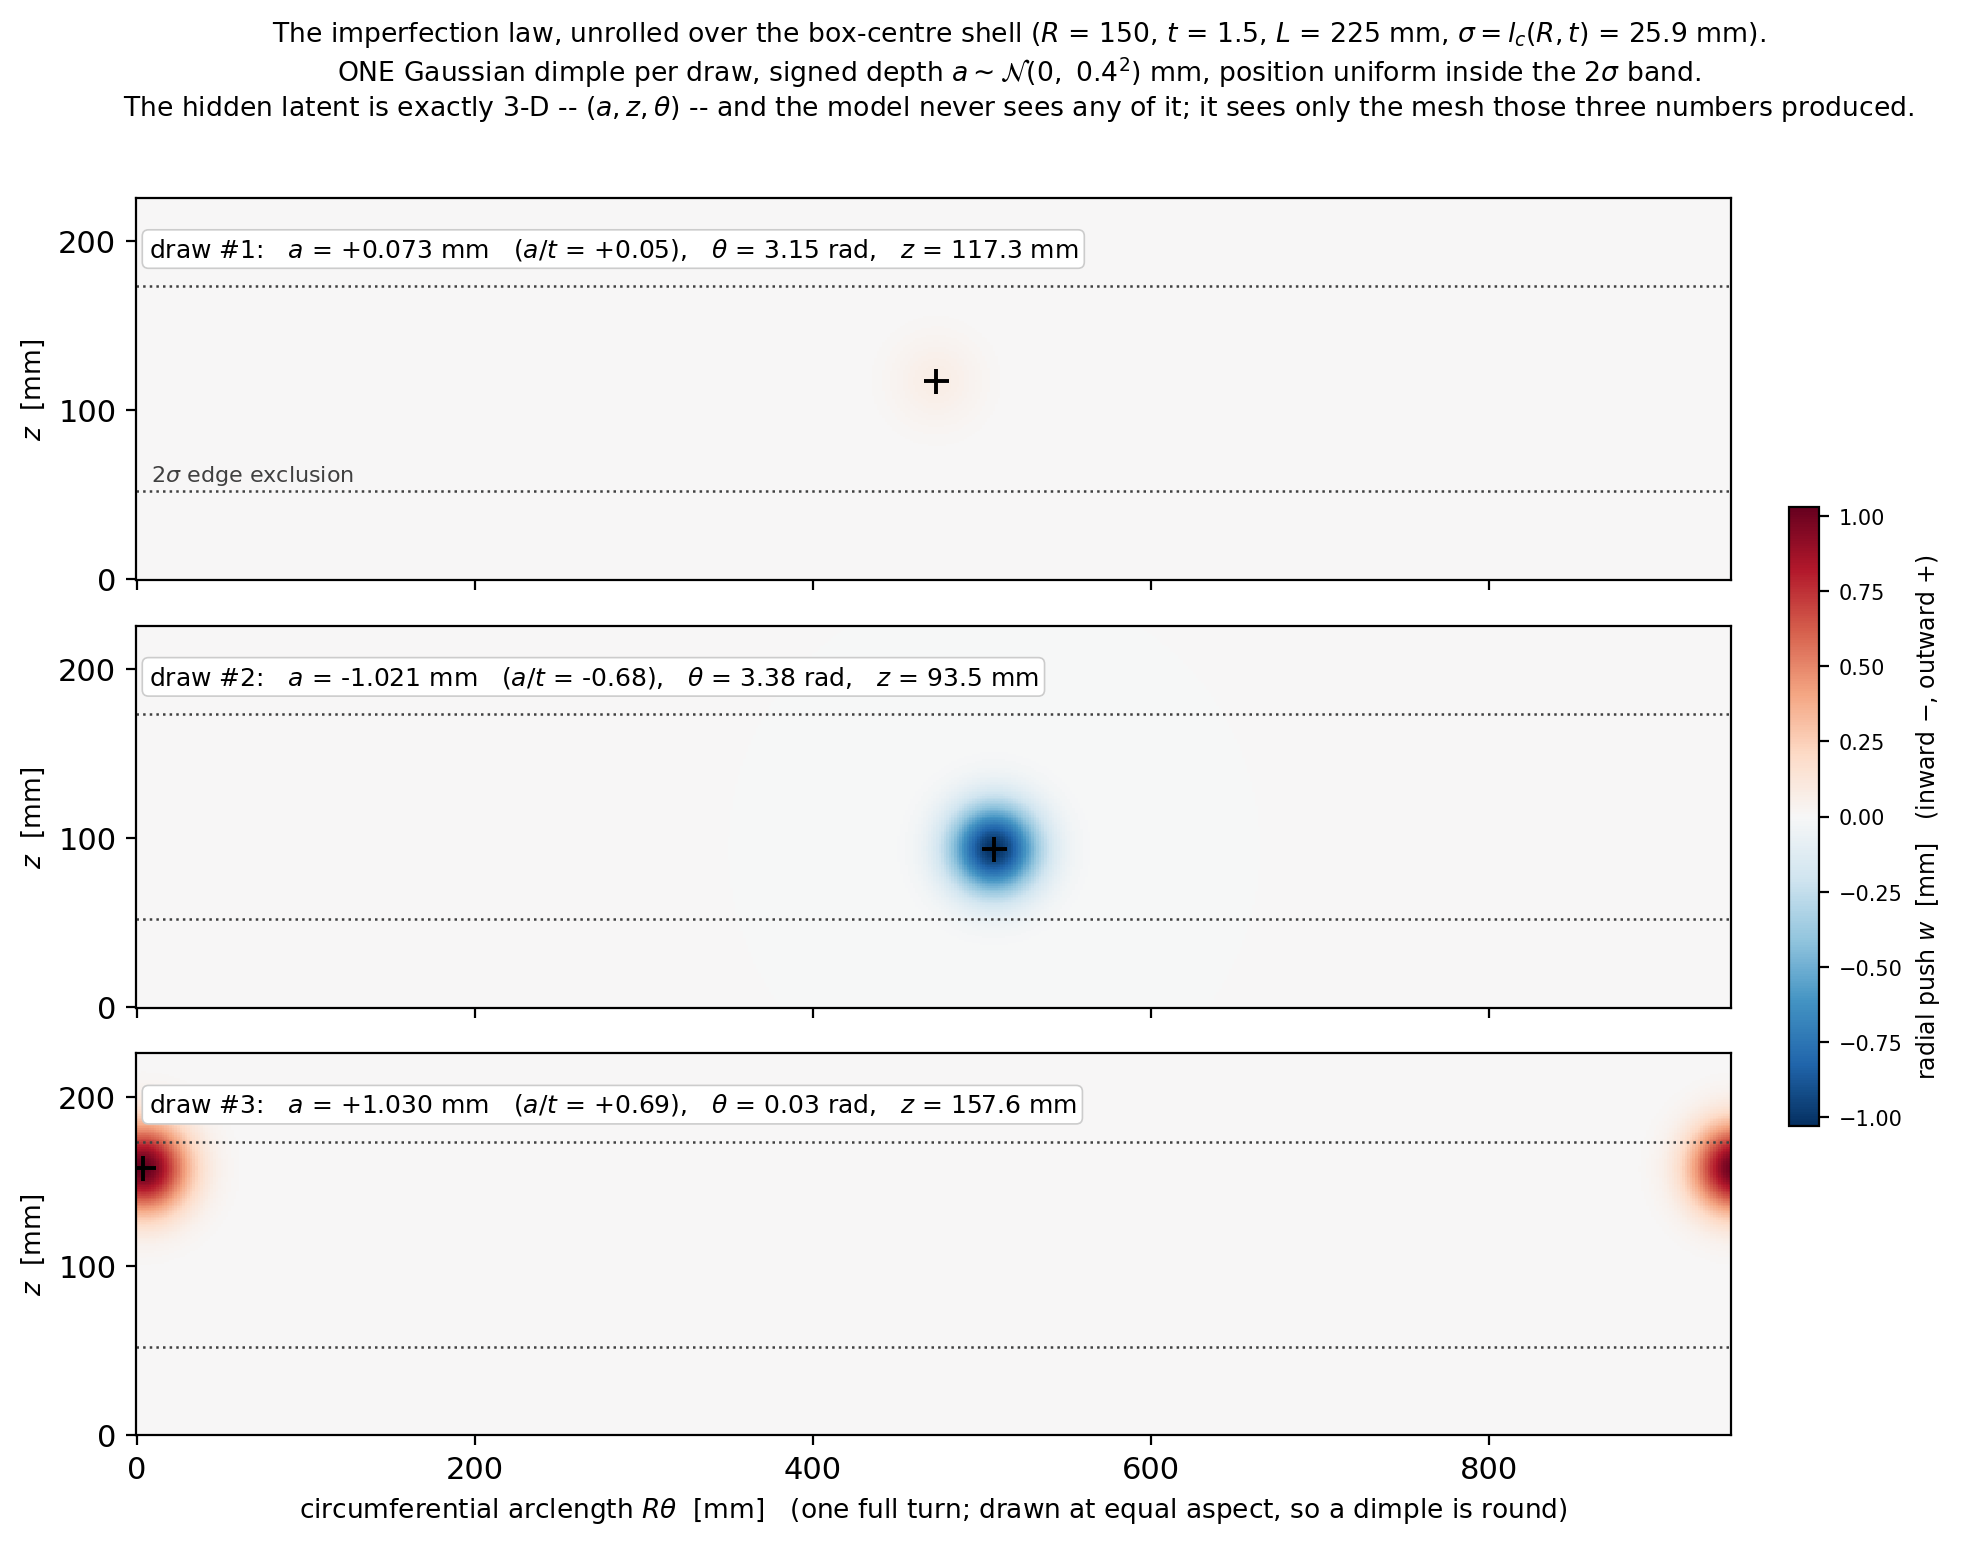
\includegraphics[width=0.78\textwidth]{figures/imperfection_dimples.png}
  \caption{같은 설계점에서 뽑은 imperfection 실현값 세 가지(다른 draw). 쉘
  표면을 펼쳐 그렸고, 가로축은 각도가 아니라 \textbf{호길이} $s = R\theta$
  --- dimple은 표면 위에서 등방(isotropic)이므로, 각도 축에 그리면 축방향
  주름처럼 잘못 보인다. 위에서부터 거의 완벽($a{=}{+}0.07$ mm), 강한 안쪽
  dimple($a{=}{-}1.02$ mm), 강한 바깥쪽 dimple($a{=}{+}1.03$ mm)이다. 점선은
  $2\sigma$ 경계 제외선. 이 그림 전체가 모델에게는 \textbf{보이지 않는다} ---
  모델이 보는 것은 완벽한 원통과 압축량 $\Delta$뿐이다.}
\end{figure}

\subsection{저장 방식: 노드 값이 아니라 dimple 목록}

Imperfection은 노드별 변위 값이 아니라 \textbf{draw마다의 dimple
목록 $\{(\theta_k, z_k, a_k)\}_{k=1}^K$와, 설계점마다 고정된 $\sigma$}로
저장한다($K{=}1$이므로 실제로는 항목 하나). 그러면 (i) 메쉬 해상도와 무관하게
어떤 노드 좌표에서든 같은 값을 식 위에서 재계산할 수 있고, (ii) "메쉬를
조밀하게 하면 imperfection이 사라지는" 함정을 원천적으로 피한다. 이 목록은
\texttt{latent/} 그룹에 저장되며, 이건 데이터셋 생성 과정을 검증하기 위한
진단용 정보일 뿐 \textbf{모델의 입력이 아니다}.

% =====================================================================
\section{3. 절차 --- 어떻게 실제로 이 imperfection이 구조 해석에 들어가는가}
% =====================================================================

\begin{enumerate}
\item \textbf{재료}: \textbf{선형탄성(linear elastic)} 등방 강재,
      $E{=}210$~GPa, $\nu{=}0.3$, $\rho{=}7.85\times10^{-6}$~kg/mm$^3$.
      단위계는 \textbf{kg-mm-ms}이므로 힘은 kN, 응력·탄성계수는 GPa,
      에너지는 J이고 $1~\mathrm{J/mm} = 1~\mathrm{kN}$이 정확히 성립한다.
      Butterfly~Defect 논문은 실제 실리콘(VPS-32)의 거동을 재현하려고
      Neo-Hookean 초탄성을 쓰지만, 이 벤치마크는 특정 소재를 재현하려는 것이
      아니라 "얇은 쉘의 극소 imperfection이 좌굴 모드를 결정한다"는
      \emph{현상 자체}를 보는 것이 목적이다. 선형탄성을 쓰는 편이 오히려 더
      일관적이다: $\sigma=l_c$ 공식(2.1절)도 $P_{cr}$ 공식(아래)도 모두
      선형(Donnell) 쉘이론에서 유도된 식이라, 그 이론이 가정하는 재료를 실제로
      쓰는 셈이 된다 --- Neo-Hookean 초탄성의 "소변형 등가 $\nu$"를 식에
      대입하는 것보다 이론적으로 맞다. 다만 이전 설계와 달리 무차원 $E{=}1$이
      아니라 \textbf{물리 단위 강재}를 쓴다: 그래야 좌굴 하중이 kN으로,
      압축량이 mm로 직접 읽히고, 하중 속도를 실제 탄성파 속도 대비로 말할 수
      있다.

      한 가지는 분명히 해둔다: \textbf{항복 곡면이 없다}(\texttt{/MAT/ELAST}).
      설계 박스에서 고전 좌굴응력 $\sigma_{cr} = 0.60523\,Et/R$은
      $0.64$--$2.54$~GPa이므로, 실제 강재라면 좌굴하기 훨씬 전에 항복한다.
      즉 이 벤치마크는 "강재로 만든 캔"의 모델이 아니라 \emph{탄성 박막쉘
      모델문제}이고, 강재의 $E$와 $\rho$는 그 모델문제에 물리 단위를 주기 위한
      선택이다. 이는 고전 좌굴이론과 knockdown factor 문헌(NASA~SP-8007 등)이
      다루는 대상과 정확히 같은 설정이므로, 보고하는 $P_{\max}/P_{cr}$은 그
      문헌과 직접 비교 가능하다. 소성까지 포함한 좌굴은 별도의 문제이며 이
      데이터셋의 범위가 아니다.
\item \textbf{메쉬}: 해석적으로 매핑된 \textbf{규칙 사각형 메쉬}이고, 요소는
      OpenRadioss의 4절점 쉘(QEPH, 두께방향 적분점 $N{=}5$)이다. 요소 차수보다
      결정적인 것은 두께방향 적분점 수였다 --- \texttt{/PROP/SHELL}의 기본값
      $N{=}1$은 굽힘 강성을 통째로 없애버려서, 완벽한 원통조차 $0.028\,P_{cr}$
      에서 무너졌다. $N{=}5$로 올리면 같은 완벽한 원통이 $1.046\,P_{cr}$에
      도달한다(사전 검증 \texttt{nint\_verify}). 메쉬 밀도는 $h \le l_c/10$
      기준으로 잡으며, 설계 박스 전체에서 $h/l_c \in [0.083,\,0.084]$,
      노드 수는 24{,}852--87{,}398(중앙값 45{,}623)이다.
\item \textbf{초기 형상}: 완벽한 원통 좌표에 dimple 변위 $w(\theta,z)$를 더한
      형상을 실제 solver의 초기 형상으로 준다. 즉 solver는 "이미 결함이 있는
      쉘"을 압축하는 셈이다. Radioss는 노드를 요소가 처음 참조한 순서로 다시
      번호 매기므로, 변형된 좌표를 쓸 때 그 순열(permutation)을 반드시 되돌려야
      한다 --- 되돌리지 않으면 최대 $112.5$ mm의 좌표 오차가 조용히 들어간다.
\item \textbf{하중}: 바닥 림은 완전 고정, 상단 림은 강체(\texttt{/RBODY})로 묶어
      축방향으로 $\Delta$만큼 눌러 내린다. $\Delta$는 파생량이 아니라 1절의
      독립 노브이며 $\mathcal{U}[1,3]$ mm에서 직접 뽑는다. 부과 방식은
      \texttt{/IMPVEL} + 상수 \texttt{/FUNCT}라서 변위 이력이 해석적으로
      닫힌 꼴이다 --- 시동 램프 없이 $\tau{=}0$부터 일정 속도 $v$로 누른다:
      \[
        \Delta(\tau) = v\,\tau,
        \qquad t_\mathrm{ramp} = 0.
      \]
      램프를 없앤 것은 의도적이다. 램프가 있으면 전달 변위가
      $v(\tau - t_\mathrm{ramp}/2)$가 되어 총 압축량에 보정항이 붙고,
      $\Delta = v\,t_{end}$라는 관계가 깨진다. 대신 $\tau{=}0$에 시동
      충격파를 하나 허용하게 되는데, 그 크기는 $\rho c v = 0.0102$~GPa로
      박스 중심 기준 $P_{cr}$의 0.8\%(14.4 kN 대 1796.8 kN)에 불과하다.
      추정에 기대지 않고 직접 A/B로 측정했다(아래 \textbf{solver와 출력 $P$}).

      비교 기준으로 쓰는 고전 임계값은 (선형 Donnell 이론, $\nu{=}0.3$)
      \[
        P_{cr} = 3.80276\,E\,t^2, \qquad
        \sigma_{cr} = 0.60523\,\frac{E\,t}{R}, \qquad
        d_{cr} = 0.60523\,\frac{t\,L}{R}
      \]
      이다. $P_{cr}$에서 $R$과 $L$이 정확히 상쇄된다는 점에 주의 --- 임계
      \emph{하중}은 두께만의 함수다. 설계 박스에서 $P_{cr}$은 798.6~kN
      ($t{=}1.0$)에서 3194.3~kN($t{=}2.0$)까지, 외삽 티어까지 포함하면
      511--4600~kN 범위다. 진단용 무차원수 $\lambda = \Delta/d_{cr}$는
      $0.44$--$3.49$에 분포한다. $\lambda$는 어디까지나 사후 진단량이고,
      샘플링을 좌우하지 않는다 --- 다섯 knob이 독립이므로 $\lambda$를 조건으로
      걸어 표본을 자르지 않는다.

      그 대가를 분명히 적어둔다: \textbf{모든 draw가 좌굴하지는 않는다}.
      학습 티어 draw의 16.7\%(25개 설계점, 1600 draw)가 $\lambda < 1$이고,
      39.3\%가 $\lambda < 1.2$다. 이런 draw는 부과한 스트로크가 끝날 때까지
      상승하는 탄성 경로 위에 머물러서, $P_{\max}$가 한계점 하중이 아니라
      \emph{스트로크 끝단의 하중}이다. 결정적으로 그 값은 \textbf{결함과
      무관하다} --- $\Delta{=}0.6$에서 서로 다른 딤플 draw 두 개가 비트 단위로
      동일한 $P_{\max}/P_{cr} = 0.442$를 돌려주었다. 따라서 이 경우
      $P_{\max}/P_{cr}$은 knockdown factor가 \emph{아니며}, 그렇게 읽으면 안
      된다. 각 draw는 한계점이 스트로크 내부에 있고($\Delta@P_{\max} <
      0.97\,\Delta$) 그 뒤로 하중이 떨어지는지($P_{\text{end}} <
      0.97\,P_{\max}$)를 판정한 불리언 \texttt{buckled} 플래그를 함께
      기록하므로, 소비자는 좌굴 라벨만 골라 쓸 수 있다.
\item \textbf{solver와 출력 $P$}: OpenRadioss의 \textbf{양함수 동해석(explicit
      dynamics)}을 그대로 쓴다. 이전 초안이 적어둔 동적 완화(\texttt{/DYREL},
      \texttt{/KEREL})는 실제 덱에 \emph{들어 있지 않다}. 그래서 준정적 조건을
      결정하는 것은 solver 설정이 아니라 오로지 \textbf{하중 속도} $v$다.

      \textbf{고정하는 것은 $t_{end}$가 아니라 $v$다.} $\Delta$ 자체가 샘플링되는
      knob이라 $[1,\,3]$~mm(외삽 티어 포함 $[0.6,\,3.6]$)를 훑으므로, $t_{end}$를
      하나로 고정하면 $\Delta{=}3$인 점이 $\Delta{=}1$인 점보다 3배 빨리 눌린다.
      아래 보듯 $P_{\max}$는 속도에 강하게 의존하므로, 이는 \emph{$\Delta$와
      상관된 편향을 라벨에 직접 써넣는} 것이 된다 --- 대리모델은 "$\Delta$가
      크면 knockdown이 높다"를 물리가 아니라 해석 일정의 산물로 학습하게 된다.
      그래서 $v = 0.25$~mm/ms를 고정하고 $t_{end}$를 점마다 다르게 둔다. 시동
      램프가 없으므로($t_\mathrm{ramp}{=}0$) 이 관계는 보정항 없이
      \[
        t_{end} = \Delta/v
        \qquad\Longleftrightarrow\qquad
        \Delta = v\,t_{end}
      \]
      로 정확히 닫힌다($\Delta{=}1,\,2,\,3$에 대해 $4,\,8,\,12$~ms).
      박스 중심에서 $v/c = 4.8\times10^{-5}$이고, 해석 시간 동안 축방향 탄성파가
      약 92회 왕복한다.

      \textbf{속도 수렴은 직접 측정했고, 완전히 수렴하지는 않았다.} 박스 중심점
      ($R{=}150$, $t{=}1.5$, $L{=}225$, $\Delta{=}2.0$)에서 두 개의 딤플 draw를
      $t_{end}$를 배로 늘려가며 다시 풀었다:

      \begin{center}
      \begin{tabular}{lrrrrr}
        \toprule
        $t_{end}$~[ms] & 1 & 2 & 4 & 8 & 16 \\
        \midrule
        $P_{\max}/P_{cr}$, $a{=}{+}0.256$~mm & 1.123 & 1.044 & 0.973 & 0.922 & 0.887 \\
        $P_{\max}/P_{cr}$, $a{=}{-}0.663$~mm & 1.005 & 0.840 & 0.735 & 0.676 & 0.684 \\
        \midrule
        KE/IE at $P_{\max}$, $a{=}{-}0.663$ & 0.032 & --- & --- & 0.0045 & 0.0016 \\
        \bottomrule
      \end{tabular}
      \end{center}

      결함이 뚜렷한 draw($a{=}{-}0.663$)는 $t_{end}{=}8$에서 이미 수렴했다
      (다음 배가에서 $+1.2$\%로, 사실상 잔차 수준). 느린 쪽은 오히려 거의
      완전한 draw($a{=}{+}0.256$)로, 분기점 근처 경로가 평탄해 좌굴 모드가
      자라는 시간이 길고 $t_{end}{=}16$에서도 아직 $-3.8$\%씩 내려간다. 즉
      \textbf{채택한 $v = 0.25$~mm/ms에서 결함이 큰 draw는 준정적이고, 거의
      완전한 draw는 수 \% 높게 남는다} --- 알려진 한계로 명시한다. 이 잔차는
      결함 크기와 상관되므로 imperfection 민감도를 약간 \emph{압축}하는
      방향이며, 과장하는 방향이 아니다. 완전 수렴에는 설계점당 $t_{end}$를
      한 자릿수 더 키워야 하고 캠페인 비용이 같은 배수로 늘어난다.

      \textbf{KE/IE는 여기서 충분한 게이트가 아니다.} 위 표의 마지막 줄이
      보여주듯, $P_{\max}$가 아직 $16$\% 부풀어 있는 $t_{end}{=}1$에서도 $P_{\max}$
      \emph{시점}의 운동/내부 에너지 비는 $0.032$로 교과서적인 5\% 기준을
      통과한다. 전역 에너지 비는 국소적인 snap-through를 보지 못하기 때문이다.
      따라서 KE/IE는 기록은 하되 준정적 판정의 근거로 쓰지 않으며, 신뢰할 수
      있는 판정은 위와 같은 직접 속도 수렴 시험뿐이다. 아울러 보고하는 값은
      \emph{해석 종료 시점}의 KE/IE가 아니라 $P_{\max}$ 시점의 값이다 --- 한계점을
      지나면 붕괴는 실제로 동적이므로 종료 시점 값은 원래 높다.

      축하중 $P$는 양쪽 림 강체의 이력(\texttt{/TH/RBODY})에서 읽는다. 여기에
      실측으로 확인한 주의점이 둘 있다. 첫째, \texttt{th\_to\_csv}는 카드에 적은
      변수 이름(\texttt{FX}/\texttt{FY}/\texttt{FZ})을 CSV 헤더로 되돌려 쓰지
      않는다 --- 채널 이름이 \texttt{rim\_forces <rbid> <title> var <N>} 형태라
      \texttt{"FZ"}로는 아무 열도 찾을 수 없다. 그래서 열은 덱에 써넣은 강체
      ID로 찾고, 카드 순서(FX,\,FY,\,FZ)의 세 번째를 축방향 채널로 쓴다.
      둘째, 그 채널에 담기는 값은 순간 하중이 아니라 \emph{누적 역적}
      $J = \int P\,dt$다. 등속 구간에서 $\int P\,dt = v^{-1}\!\int P\,d\Delta$이므로
      $J\,v$가 $\mathrm{EXT\text{-}WORK}$와 일치해야 하는데, 실제로 해석 전
      구간에서 0.1\% 이내로 일치한다. 이를 하중으로 잘못 읽으면 크기가 약 2배
      작고 한계점 없이 단조 증가하는 곡선이 나온다. 따라서 $P = dJ/dt$로
      미분해서 쓴다. 이미 적분량이라 미분은 잘 조건화되어 있다: 2차 차분의
      rms가 5.1~kN(최대 하중 2018~kN 대비 0.25\%)이고 3점 평활을 걸어도
      $P_{\max}$가 0.08\%밖에 움직이지 않는다. 그래서 평활 없이 그대로 미분한다.

      결과적으로 $P_{\max}$를 서로 독립인 세 경로로 얻는다: (i) 고정된 바닥
      림의 반력 $dJ_{\mathrm{bot}}/dt$(주 경로), (ii) 구동되는 상단 림의 반력
      $dJ_{\mathrm{top}}/dt$(평형 점검), (iii) 에너지 수지
      $d(\mathrm{EXT\text{-}WORK})/d\Delta$를 TH 샘플링 레이트(200점)에서 미분한 값.
      세 값은 박스 중심점에서 0.06\%, 12개 draw 전체에서 1.48\% 이내로 일치한다.
      세 경로 모두 맨 앞 두 샘플은 빼고 최댓값을 취한다 --- $\Delta(0){=}0$이라
      $t{=}0$의 편측 차분 $dW/d\Delta$가 $0/0$이 되고, 한계점은 어차피 훨씬 뒤에
      있다. 보고하는 knockdown factor는 $P_{\max}/P_{cr}$이다.
\end{enumerate}

% =====================================================================
\section{4. 예상 출력(Output) --- 데이터셋에 실제로 무엇이 담기는가}
% =====================================================================

\subsection{하나의 "샘플"이 무엇인가}

하나의 설계점(design point)에 대해, dimple 실현값을 여러 번 독립적으로 뽑아
여러 번 해석을 돌린다. 즉 데이터셋의 기본 단위는

\begin{center}
설계점 $(R,t,L,\Delta)$ $\;\longrightarrow\;$ \{ solve(dimple 실현값\textsubscript{1}), \ldots, solve(dimple 실현값\textsubscript{64}) \}
\end{center}

이며, 같은 설계점 안의 64개 draw는 입력 쪽에서는 \textbf{완전히 구분 불가능}하고
(전부 같은 완벽한 원통 좌표와 같은 $\Delta$를 본다), 출력 쪽에서만 서로 다른
최종 변위장과 서로 다른 $P_{\max}$를 갖는다. 이게 성립해야 "one-to-many"라는
주장이 성립한다 --- 그리고 이건 데이터를 만들고 나서 반드시 직접 확인해야
하는 것이지, 설계만으로 보장되지 않는다(3절의 준정적 조건이 잘못되면 사실상
하나의 결과만 나올 수 있다).

\subsection{실제 렌더링: 학습 형상 10개의 원본과 최종 변형}

\noindent
\textbf{주의: 아래 그림은 이전(4-티어 $R/t\times L/R$) 캠페인에서 렌더링한
것이다.} 5-노브 설계로 다시 돌린 캠페인이 끝나면 같은 스크립트로 재렌더링하여
교체한다 --- 그때까지는 렌더링 파이프라인이 동작한다는 증거로만 읽어야 하고,
여기 찍힌 형상 값 자체는 현재 설계 박스의 것이 아니다.

\begin{figure}[h]
  \centering
  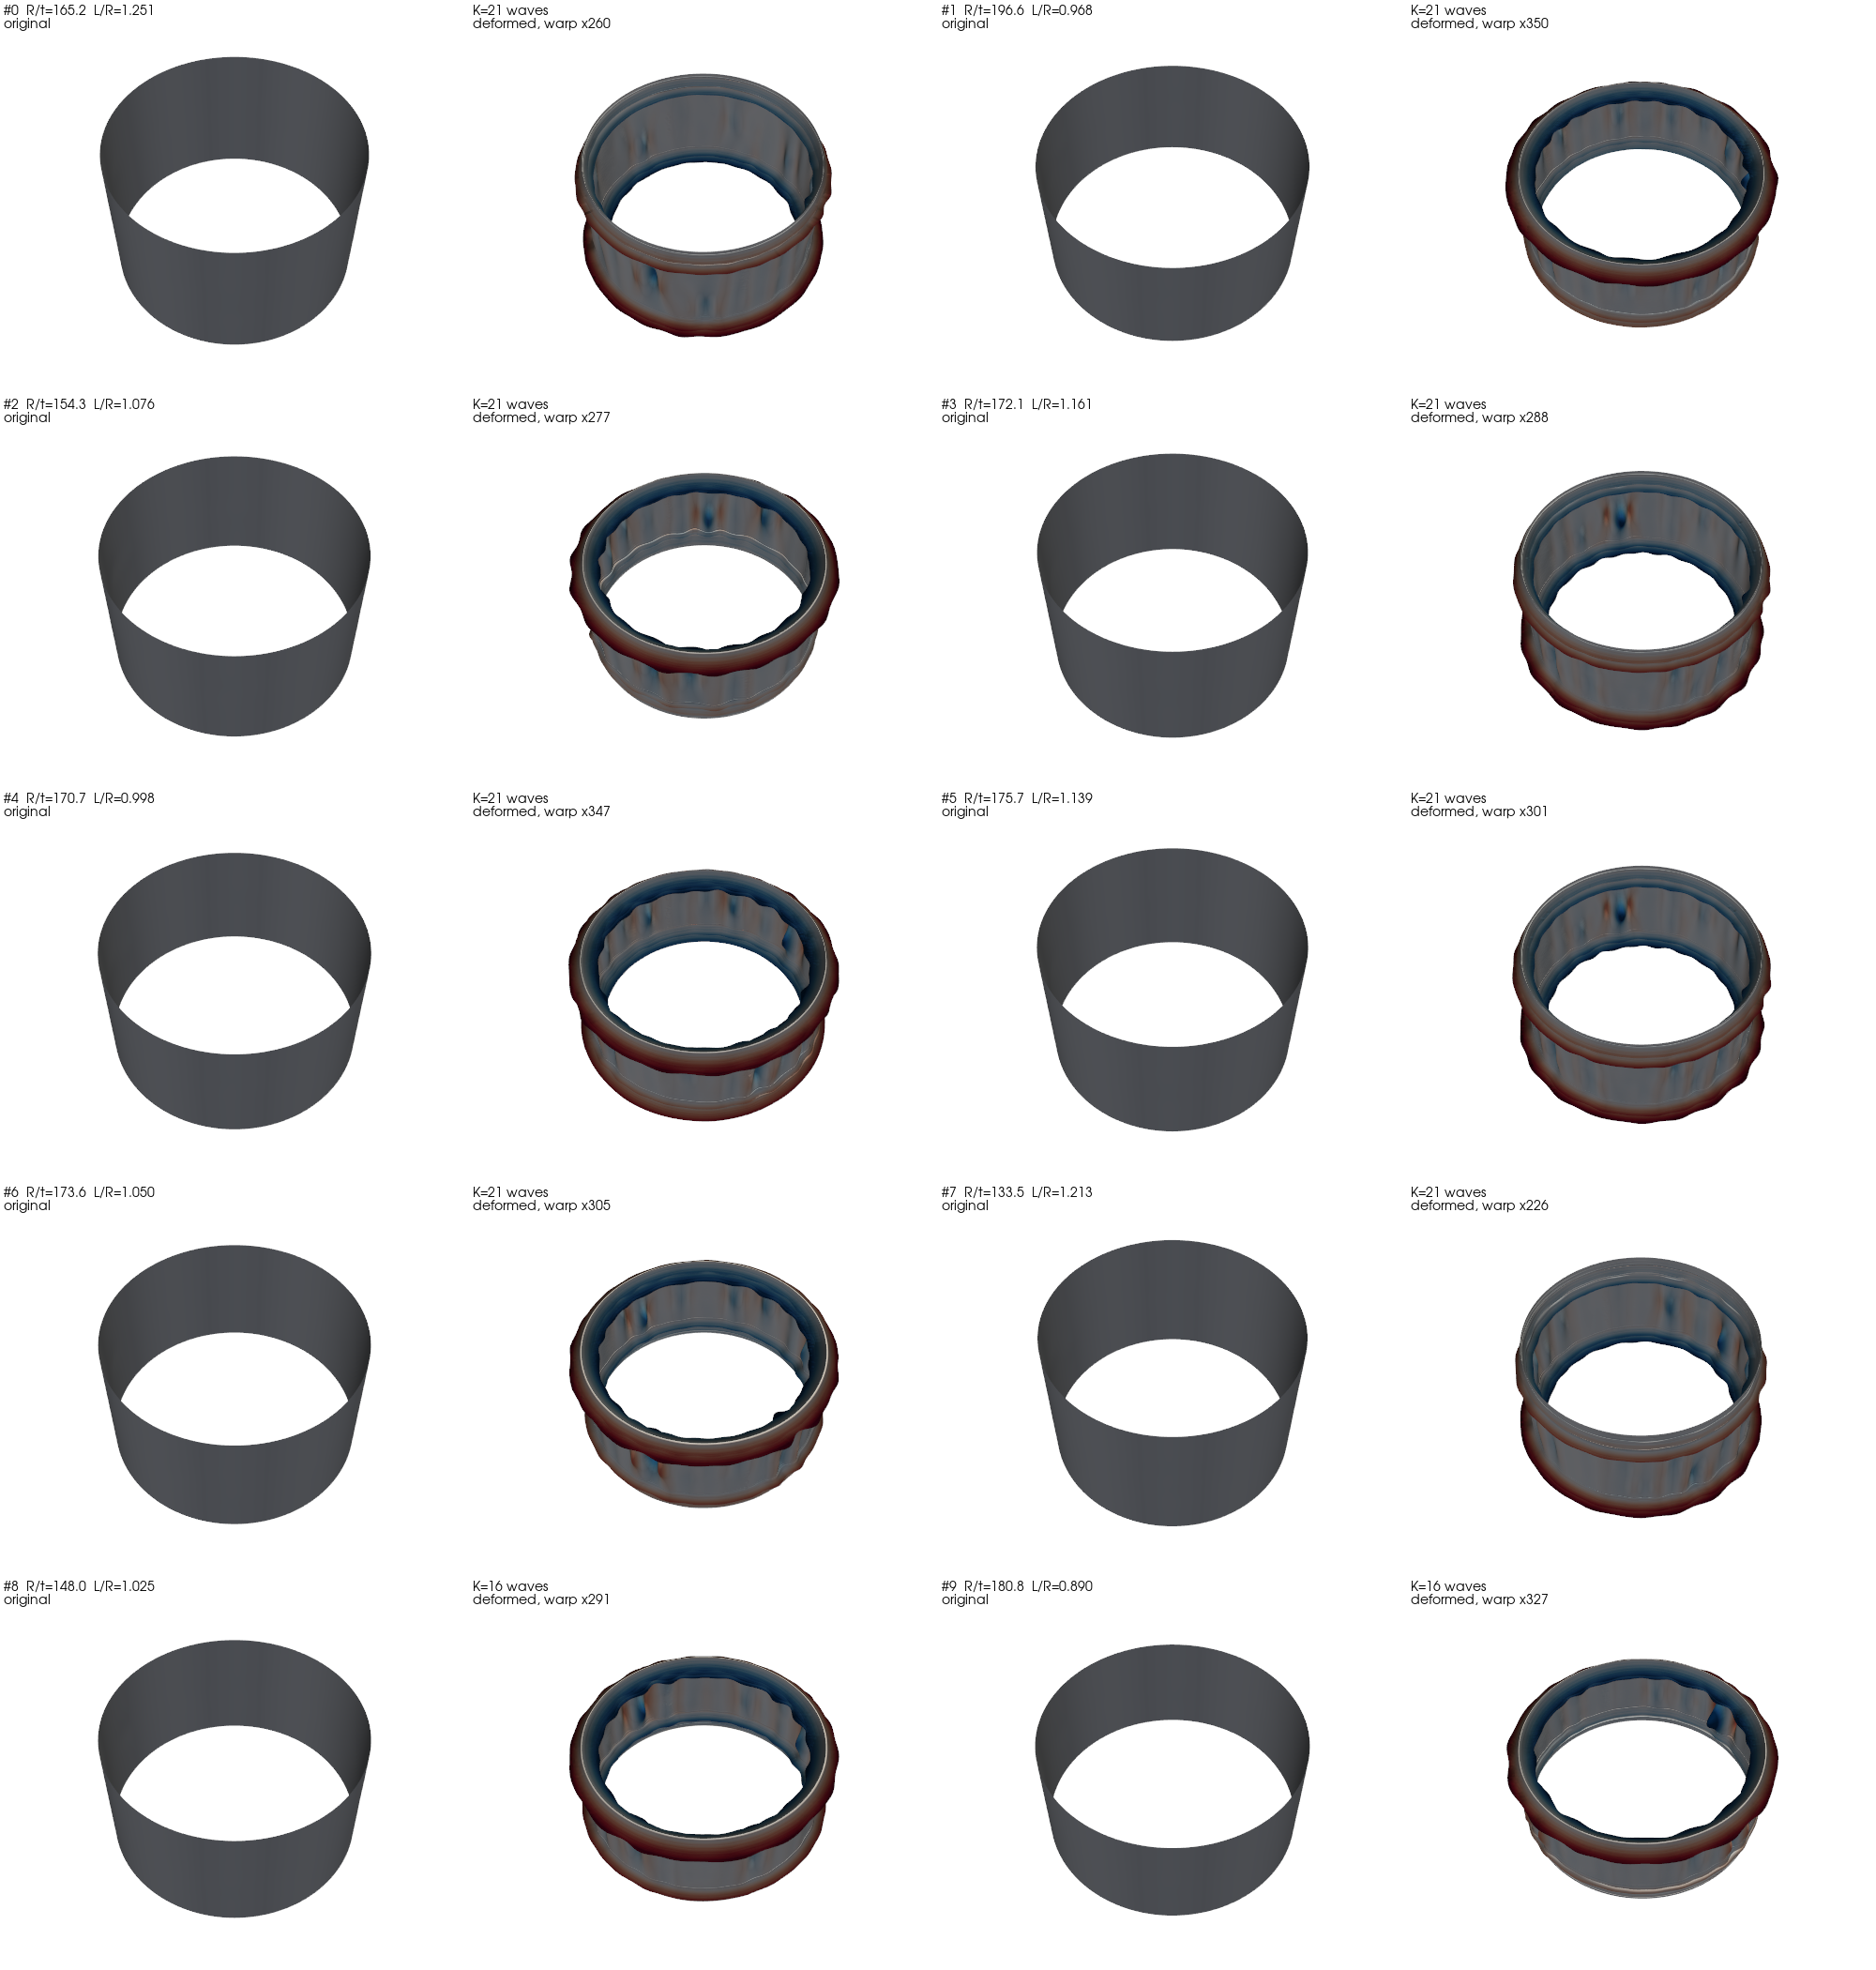
\includegraphics[width=0.98\textwidth]{figures/sample_geometries_orig_deformed.png}
  \caption{\emph{(이전 캠페인 렌더링 --- 재생성 대기)} 학습 형상 10개(\#0--\#9),
  각각 대표 draw(seed 0) 하나씩. 왼쪽 패널은 원본(완벽한 원통, $t{=}0$ ANIM 프레임),
  오른쪽 패널은 최종 변형($t{=}t_\mathrm{end}$ ANIM 프레임)이며 색은 반경
  방향 변위 $r(t_\mathrm{end})-r(t{=}0)$를 나타낸다. 실제 좌굴 후 반경
  변위는 반경 $R$의 몇 퍼센트에 불과해 눈에 보이지 않으므로, 기하학적으로만
  x226--x350배 과장했다(패널마다 표시된 배율; 색 스케일 자체는 과장하지
  않은 실제 값이다). 각 패널의 물결 개수가 그 형상 draw의 좌굴 모드
  $K$(요약 로그에 기록된 값)와 일치한다 --- OpenRadioss의 \texttt{ANIM}
  바이너리를 벤더 제공 \texttt{anim\_to\_vtk} 변환기로 VTK로 바꾼 뒤
  PyVista로 렌더링했다. 같은 형상 안에서 draw마다 달라지는 것(이 절의
  핵심 주장)은 이 그림이 아니라 통계적 분포로 별도 확인했다 --- 여기 있는
  10개는 형상 \emph{간} 다양성만 보여준다.}
\end{figure}

\subsection{HDF5에 저장되는 행(row)}

\begin{table}[h]
\centering
\small
\begin{tabular}{@{}clc@{}}
\toprule
행(row) & 내용 & 역할 \\
\midrule
0:3  & 완벽한 원통의 기준 좌표 & 입력 (절대 예측 대상 아님) \\
3:6  & 최종 변위 $(u_x, u_y, u_z)$ & \textbf{출력} \\
6    & 노드 두께 $t$ & 입력만 (조건) \\
7    & 부과 압축량 $\Delta$ (노드마다 같은 값) & 입력만 (조건) \\
8    & 노드 타입 (0 내부 / 1 고정단 / 2 하중단) & 입력만 (조건) \\
\bottomrule
\end{tabular}
\caption{HDF5 저장 계약, 총 9개 행: \texttt{input\_var}$=3$,
\texttt{output\_var}$=3$, \texttt{cond\_var}$=3$. 행 6--8이 입력 전용 조건
행이며, 노드 타입은 스위트 규약대로 \textbf{항상 마지막 행}이다. $\Delta$가
여기 들어가는 이유는 1절의 다섯 노브 중 넷이 설계점 속성이기 때문이다 ---
$R,t,L$은 좌표(행 0:3)와 두께(행 6)에서 이미 복원되지만, $\Delta$는 어느
행에서도 읽히지 않으므로 별도로 실어야 모델이 하중 조건을 볼 수 있다. 기하는
같고 $\Delta$만 다른 두 draw는 정답이 완전히 다르기 때문에, 이 행이 빠지면
one-to-many가 아니라 그냥 \emph{설명 불가능}한 데이터가 된다. Dimple 목록
$\{\theta_k,z_k,a_k\}$과 $\sigma$, 그리고 측정된 $P(\Delta)$ 이력은 이 표에
없는 별도의 \texttt{latent/} 그룹에 저장되며, 모델이 읽는 입력 행에는 절대
포함되지 않는다.}
\end{table}

\subsection{"성공"은 어떻게 판단하는가}

MGN-V가 이 벤치마크를 통과한다는 것은, 하나의 held-out 형상에 대해 모델이
샘플링한 필드들의 앙상블이, 실제 FEA로 만든 독립적인 필드 앙상블과
\textbf{분포 수준에서} 비슷하다는 뜻이다. 구체적으로:

\begin{itemize}
\item 단순 MSE(평균 오차) \textbf{하나만으로는} 판단할 수 없다 --- 여러 모드 중
      평균만 맞히는 모델과 실제로 여러 모드를 재현하는 모델이 MSE로는
      구별되지 않을 수 있다.
\item 대신 energy score / CRPS 같은 proper probabilistic score로, 모델
      앙상블 대 진짜 FEA 앙상블을 직접 비교한다.
\item 보조 진단으로 원주 방향 변위 스펙트럼(어느 모드 번호 $n$이 우세한가)을
      함께 본다 --- 다만 이건 학습 목표가 아니라 사후 분석용이다. 이전 프로젝트에서
      이미 확인된 사실: argmax 모드 번호 하나만으로는 정보가 손실된다(어떤
      형상 쌍은 필드로는 구분되지만 모드 번호로는 구분되지 않았고, 근접-퇴화
      draw의 1/6은 수치 감쇠 계수만 바꿔도 모드 번호가 뒤집혔다). 그래서 전체
      필드/스펙트럼을 그대로 내보내고, 라벨은 참고용으로만 쓴다.
\end{itemize}

% =====================================================================
\section{5. 참고 연구와의 비교: Butterfly Defect (arXiv:2607.19245)}
% =====================================================================

이 벤치마크의 물리적 직관과 방법론 --- "얇은 쉘의 축좌굴은 극소 imperfection이
모드를 결정한다"는 것과 국소 Gaussian dimple을 RSA로 배치하는 방식 --- 은
모두 EPFL/Harvard 공동 연구인 Butterfly~Defect 논문에서 가져왔다. 아래 표는
어느 부분이 정확히 같고 어느 부분이 다른지를 항목별로 검증한 결과다.
Imperfection의 \emph{형태}(Gaussian dimple)와 \emph{폭의 크기법칙}($\sigma=l_c$)은
원본 논문의 수식을 그대로 재사용하지만, 재료는 원 논문의 Neo-Hookean 초탄성이
아니라 물리 단위 선형탄성 강재를 쓰고, 설계 공간의 철학(파생 무차원수 스윕 대
5개 독립 노브), 결함 개수($N\gg1$ 대 $K{=}1$), 진폭 분포(정규화 로그정규 대
물리 단위 정규), 배치 제외 영역($3\sigma$ 대 $2\sigma$)은 의도적으로 다르게
설계했다. 가장 근본적인 차이는 imperfection의 \textbf{가시성}(모델이 볼 수
있는가)과 \textbf{출력의 형식}(스칼라 대 전체 분포)이다 --- 이 둘이 바로 이
벤치마크가 존재하는 이유다.

\begin{longtable}{@{}p{2.6cm}p{5.4cm}p{5.4cm}@{}}
\toprule
 & \textbf{Butterfly Defect (원본 논문)} & \textbf{이 벤치마크} \\
\midrule
\endhead
설계 공간 (범위) &
  $R/t \in [20, 1500]$, 10개의 개별 다중결함 형상(재료·기하가 각각 실험마다
  다름) &
  \textbf{다름}: 원통 하나의 형상족, 물리 단위 4차원 박스
  $R\in[100,200]$, $t\in[1,2]$, $L\in[150,300]$, $\Delta\in[1,3]$ mm 위의
  LHS 150점 + 한 축씩 외삽한 t1 8점 = 158 설계점 \\
\addlinespace
설계 공간 (철학) &
  Batdorf 파라미터 $Z=H^2\sqrt{1-\nu^2}/(Rt)$를 \textbf{고정}($Z{=}2771$)한
  채 $R,H,t$만 바꿔서 표면적(=결함 개수 $N$)을 바꾼다 --- 좌굴 거동의
  ``종류''는 고정하고 결함 통계만 바꾸는 설계 &
  \textbf{다름}: 무차원 파생량($Z$, $R/t$, $L/R$)을 스윕하지 \emph{않는다}.
  우리가 정하는 것은 실제로 손에 잡히는 치수 다섯 개뿐이고, 모두 하나의
  박스 위 독립 분포다 --- 조건부 경계도 기각도 없다. 파생량은 전부 사후
  진단으로만 본다 \\
\addlinespace
하중 제어 &
  하중 제어에 해당(출력이 임계하중 $P_{cr}$) &
  \textbf{다름}: \textbf{변위 제어}. 극한점 이후에는 평형이 없어 하중 제어가
  성립하지 않으므로, 압축량 $\Delta$를 부과하고 $P$를 강체 반력에서 읽는다
  --- $P$는 노브가 아니라 출력 \\
\addlinespace
재료 &
  Neo-Hookean 초탄성 (VPS-32 실리콘, $C_{10}=G/2=0.21\,\mathrm{MPa}$,
  $D_1{=}0$, $E=1.26\,\mathrm{MPa}$, $\nu{=}0.5$) &
  \textbf{다름}: Neo-Hookean 초탄성이 아니라 \emph{선형탄성(linear
  elastic)} 등방 \textbf{강재} --- $E{=}210$~GPa, $\nu{=}0.3$,
  $\rho{=}7.85\times10^{-6}$~kg/mm$^3$ (kg-mm-ms). $l_c$ 공식(2.1절)도
  $P_{cr}$ 공식도 선형 쉘이론(Donnell)에서 유도된 식이라 재료 모델과의
  정합성이 오히려 더 높고, 물리 단위라서 kN·mm로 직접 읽힌다 \\
\addlinespace
Imperfection 수식의 형태 &
  일반형은 \textbf{이방성} 타원 Gaussian (Eq.~4): 진폭 $\delta_i$, 종횡비
  $a_i$(원주/축 폭 비), 크기 $\lambda_i$ 세 모양 파라미터를 가짐 &
  \textbf{부분적으로 동일}: 등방(원형) Gaussian만 구현 --- 다만 원 논문의
  확률적 앙상블도 $a{=}1,\lambda{=}1$로 고정해 쓰므로($l_x{=}l_z{=}l_c$),
  \emph{그 특정 경우}에서는 원 논문의 식도 등방이 되어 우리 식과 정확히
  일치한다. 우리가 구현하지 \emph{않은} 것은 $(a,\lambda)$를 바꾸는
  결정론적 스윕(Sec.~IV)뿐 \\
\addlinespace
Imperfection 폭의 크기법칙 &
  $\sigma = l_c = \pi[12(1-\nu^2)]^{-1/4}\sqrt{Rt}$ (Eq.~3, 고전적 축대칭
  좌굴 반파장 --- $R,t$ 둘 다에 의존) &
  \textbf{동일}: $\sigma = l_c$를 그대로 재사용(2.1절) --- 처음에는
  $\sigma=0.11R$($t$에 무관)로 잘못 단순화했다가, 이번 검토에서 $R/t$가
  커질수록(얇은 쉘일수록) 원 논문의 $l_c/R$은 줄어드는데 $0.11R$은 그대로
  라는 불일치를 발견하고 수식 자체를 $l_c(R,t)$로 고쳤다 \\
\addlinespace
위치 배치 &
  $(\theta,z)$ 균일분포 + RSA, 최소 분리거리 $2\,l_c$ &
  \textbf{동일(단, 무의미해짐)}: 균일분포 + RSA 구현을 그대로 두지만
  $K{=}1$이라 최소 분리거리 조건이 발동할 상대가 없다 --- 실질적으로
  ``표면 위 균일, 양 끝 $2\sigma$ 제외'' \\
\addlinespace
진폭 분포 &
  로그정규분포, 정규화 진폭 $\bar\delta{=}a/t$ 기준
  $\langle\bar\delta\rangle{=}0.15$, $\Delta\bar\delta{=}0.05$ (부호 $\pm$ 랜덤) &
  \textbf{다름}: 물리 단위 정규분포 $a \sim \mathcal{N}(0,\,0.4^2)$ mm.
  $a/t$로 뽑으면 깊이가 두께에 종속되어 노브의 독립성이 깨지므로 mm로 직접
  뽑고, 부호는 정규분포의 대칭성에서 자동으로 반반 나온다. 결과적으로
  $|a|/t$는 중앙값 $0.178$, p99 $0.666$으로 원 논문의 스케일 대역을 덮는다 \\
\addlinespace
결함 개수 $K$/$N$ &
  세 체제를 \textbf{각각} 실험: $N{=}1$(결정론적, Sec.~IV), $N{=}2$(쌍
  상호작용, Sec.~V), $N\gg1$(확률적 다중결함, Sec.~VI, 포화까지 스윕) &
  \textbf{다름}: $K{=}1$ 고정. 원 논문의 첫 번째 체제와 같은 개수지만 용도가
  반대다 --- 원 논문은 $N{=}1$을 \emph{결정론적} 스윕으로 쓰고, 우리는 그
  하나의 결함을 \emph{숨겨서} 잠재변수를 정확히 3차원 $(a,z,\theta)$으로
  만드는 데 쓴다(5.1절) \\
\addlinespace
결함 배치 제외 영역 &
  두 가지 구성을 \textbf{비교}: 전체 표면(제외 없음) vs. mid-band
  $z\in[-H/4,H/4]$ --- 경계 효과와 결함-결함 상호작용을 분리하기 위한 대조
  실험 &
  \textbf{다름}: 고정단·하중단 근처 $2\sigma$ 폭만 배제하는 단일 규칙 하나
  뿐이며, 원 논문처럼 두 구성을 비교하지는 않는다. $2\sigma$인 이유는
  $3\sigma$가 설계 박스의 짧은 구석에서 성립하지 않아 기각을 도입해야 하기
  때문이다(2.2절) \\
\addlinespace
Imperfection의 가시성 &
  실현값 자체가 실험의 \textbf{입력 파라미터} (해당 논문의 목적상 당연히 알아야 함) &
  \textbf{다름(핵심 설계 지점)}: 실현값(dimple 목록)은 모델에게
  \textbf{숨김} --- 이게 이 프로젝트 전체의 존재 이유 \\
\addlinespace
Solver &
  Abaqus/Standard(2023), S4R 쉘(4절점 축소적분), arc-length(Riks) &
  \textbf{다름(실용적 이유)}: OpenRadioss \textbf{양함수 동해석}, 4절점
  쉘(QEPH, 두께방향 적분점 $N{=}5$), 속도 램프로 부과한 변위. 무료 solver에
  arc-length가 없어서이며, 준정적 조건은 하중 속도를 $v = 0.25$~mm/ms로 고정하고
  ($v/c = 4.8\times10^{-5}$) 그 속도에서의 수렴을 직접 측정해 확보한다. 3절이
  적어둔 대로 완전 수렴은 아니다 \\
\addlinespace
주 출력 &
  스칼라 knockdown factor $\kappa = P_{cr,\text{imperfect}}/P_{cr,\text{perfect}}$ &
  \textbf{다름(핵심 설계 지점)}: 전체 3차원 변위장의 \textbf{분포} (스칼라
  하나가 아니라 분포 자체가 목표). $\kappa = P_{\max}/P_{cr}$도 함께 기록하되
  진단용이다 \\
\addlinespace
규모 &
  20,000+ 시뮬레이션, 형상당 200회, 형상 10개 &
  \textbf{다름}: 158 설계점 $\times$ 64 draw $=$ 10{,}112 draw
  (train 150점 + t1 8점) \\
\bottomrule
\caption{원본 논문과 이 벤치마크의 설계 차이를 상세 비교한 표. Imperfection의
\emph{형태}(등방 Gaussian dimple)와 \emph{폭의 크기법칙}($\sigma=l_c$)은 검증
후 정확히 계승했다. 나머지는 의도적으로 다르다: 재료는 물리 단위 선형탄성
강재, 설계 공간은 무차원 파생량 스윕이 아니라 치수 다섯 개의 독립 박스, 하중은
변위 제어($P$는 출력), 결함은 $K{=}1$, 진폭은 mm 단위 정규분포, 제외 영역은
$2\sigma$다. 남은 근본적인 차이는 --- 애초에 이 벤치마크가 존재하는 이유인 ---
imperfection의 가시성과 출력 형식(분포 대 스칼라) 두 곳이다.}
\end{longtable}

\subsection{왜 dimple을 하나로 줄였는가 --- sparse의 극단}

Butterfly~Defect 논문의 데이터에는 흥미로운 규칙이 있다: 결함 개수 $N$이
많아질수록(다중결함 앙상블이 "포화"될수록) 결과의 변동계수(CoV) $\omega_\kappa$가
지수적으로 감소해서 거의 결정론적인 값($\kappa_0 \approx 0.61$)으로 수렴한다
(Eq.~6--7). 원 논문이 전체표면 구성에서 실측으로 맞춘 특성 개수는
$N_0 \approx 427$($\kappa$가 꺾이는 스케일)과 $N_1 \approx 186$
($\omega_\kappa$가 지수적으로 꺾이는 스케일)이다 --- 즉 "포화되어 거의
결정론적"이라 부를 만한 영역은 대략 $N$이 수백 개 수준부터다. 반대로 결함이
드문(sparse) 영역에서는 CoV가 훨씬 크게 유지된다. 우리에게 필요한 건 정확히
후자다 --- "출력이 진짜로 다양하게 갈리는" 영역이어야 one-to-many 벤치마크로서
의미가 있다.

$K{=}1$은 그 sparse 방향으로 갈 수 있는 \textbf{끝}이다. 원 논문의 CoV
감쇠식($\omega_\kappa(N)/\omega_0 = \exp[-(N/N_1)^q]$, 전체표면 구성
$\omega_0{=}0.083$, $N_1{=}186$, $q{=}0.19$)에 $N{=}1$을 넣으면 $\approx0.71$로,
$N{=}20$의 $\approx0.52$나 $N{=}40$의 $\approx0.47$보다 오히려 산포가 크다.
즉 dimple을 줄이는 방향은 one-to-many를 약화시키는 게 아니라 \emph{강화}한다.
물리적으로도 당연하다 --- 좌굴 개시는 결국 가장 불리한 결함 \emph{하나}가
결정하고, 결함이 많아질수록 "가장 불리한 하나"의 통계가 평균으로 수렴하면서
결과가 결정론적으로 굳는다. 실제로 사전 검증(\texttt{k1\_verify})에서 $K{=}1$이
knockdown 산포를 그대로 만들어낸다는 것을 확인했다.

$K{=}1$을 고른 진짜 이유는 따로 있다. 개수를 하나로 고정하면 숨겨진
잠재변수가 정확히 3차원 $(a, z, \theta)$이 된다. $K$ 자체를 확률변수로 두면
잠재공간의 \emph{차원}이 draw마다 바뀌어서, "모델이 못 보는 모호함이 몇
차원인가"라는 질문에 애초에 답이 없어진다 --- 생성모형의 잠재 용량을
평가하려는 벤치마크에서는 치명적인 모호함이다. 3차원으로 고정하면 반대로
모든 게 명확해진다: 모델이 뽑아야 할 분포는 3차원 잠재변수가 유도하는
필드 분포이고, 그 3차원의 분포는 우리가 정확히 알고 있으며(2.2절),
$\Delta$까지 입력으로 주므로 나머지 모든 입력 모호함은 제거되어 있다.

% =====================================================================
\section{요약}
% =====================================================================

\begin{itemize}
\item \textbf{다섯 개의 노브}: $R\!\sim\!\mathcal{U}[100,200]$,
      $t\!\sim\!\mathcal{U}[1,2]$, $L\!\sim\!\mathcal{U}[150,300]$,
      $\Delta\!\sim\!\mathcal{U}[1,3]$ mm (설계점마다), $a\!\sim\!\mathcal{N}(0,0.4^2)$
      mm (draw마다). 하나의 박스 위 독립 분포 --- 조건부 경계도, 기각도,
      파생 무차원수 스윕도 없다. LHS 150점 $+$ 한 축씩 외삽한 t1 8점
      $=$ 158 설계점, 설계점당 64 draw, 총 10{,}112 draw.
\item \textbf{$P$는 입력이 아니라 출력}: 극한점 이후엔 평형이 없으므로 변위
      제어로 밀고, 축하중은 상단 강체의 반력 이력(\texttt{/TH/RBODY})에서
      읽는다. 보고값은 $P_{\max}/P_{cr}$이며 $P_{cr}=3.803\,E\,t^2$.
\item \textbf{Imperfection}: 단 하나의 법칙, 단 하나의 dimple($K{=}1$).
      깊이 $a$는 mm 단위 정규분포(부호가 안쪽/바깥쪽), 위치는 표면 위 균일
      (양 끝 $2\sigma$ 제외), 폭 $\sigma=l_c(R,t)$는 설계점마다 고정.
      숨겨지는 잠재변수는 정확히 3차원 $(a,z,\theta)$이고, 이게
      one-to-many의 유일한 원천이다.
\item \textbf{재료}: 선형탄성 강재, $E{=}210$~GPa, $\nu{=}0.3$,
      $\rho{=}7.85\times10^{-6}$~kg/mm$^3$ (kg-mm-ms 단위계, 힘은 kN) ---
      원 논문의 Neo-Hookean 초탄성이 아니며, 이전 초안의 무차원 $E{=}1$도
      아니다.
\item \textbf{출력}: 최종 3차원 변위장 \emph{분포} (스칼라 knockdown factor 아님),
      energy score/CRPS로 앙상블 대 앙상블 비교. HDF5는 9행 계약
      (좌표 3 $+$ 변위 3 $+$ 조건 3: 두께, $\Delta$, 노드 타입).
\item \textbf{원본 논문과의 관계}: Imperfection의 \emph{형태}(등방 Gaussian
      dimple)와 \emph{폭의 크기법칙}($\sigma=l_c$)은 검증 후 정확히 계승했다.
      재료, 설계 공간의 철학, 하중 제어 방식, 결함 개수, 진폭 분포, 제외
      영역 폭은 의도적으로 다르게 설계했다(5절 표 참고). 근본적인 차이는
      imperfection의 가시성(숨김 대 입력)과 출력 형식(분포 대 스칼라) 두
      곳이다.
\end{itemize}

솔버 세부 사항(OpenRadioss 덱 작성, 준정적 판정 기준, 파일럿 절차)은 별도 문서
\texttt{docs/research/shell\_buckling/OPENRADIOSS\_BUILD\_PLAN.md}에서 다룬다.

\end{document}
